%!TEX root = ../main.tex

\section{Design} % (fold)
\label{sec:design}

In this chapter we will look at the design of the prototype, which will be used in our test with the purpose of answering the final problem statement. 
The design will be based on the list of requirements (see chapter \ref{sec:list_of_requirements} for the list of requirements). 
We are also going to take a look at the delimitation of our weather categories (e.g. temperature, wind speed, precipitation...). 
Based on the requirements and delimitation, pre-tests will be designed and carried out. 
These tests will then lead into a design blueprint of our prototype.

From the list of requirements it should be possible to plan how the prototype is going to fulfil all of the specific requirements. 
Additionally, the weather categories have to be delimited into a realistic amount of weather conditions which suits our timetable. 
After the delimitation, the visual and auditory elements will be chosen from the results of pre-testing, whereof the pre testing determines the sounds and visual elements which will later be used in the actual implementation. 
When the sounds and pictures are in place, it is time to create the blueprint of what the pictures should look like and how the sounds are going to be made. 
Figure~\ref{fig:design1} describes the process of the actual design of the prototype.

\begin{figure}[!htbp]
    \centering
    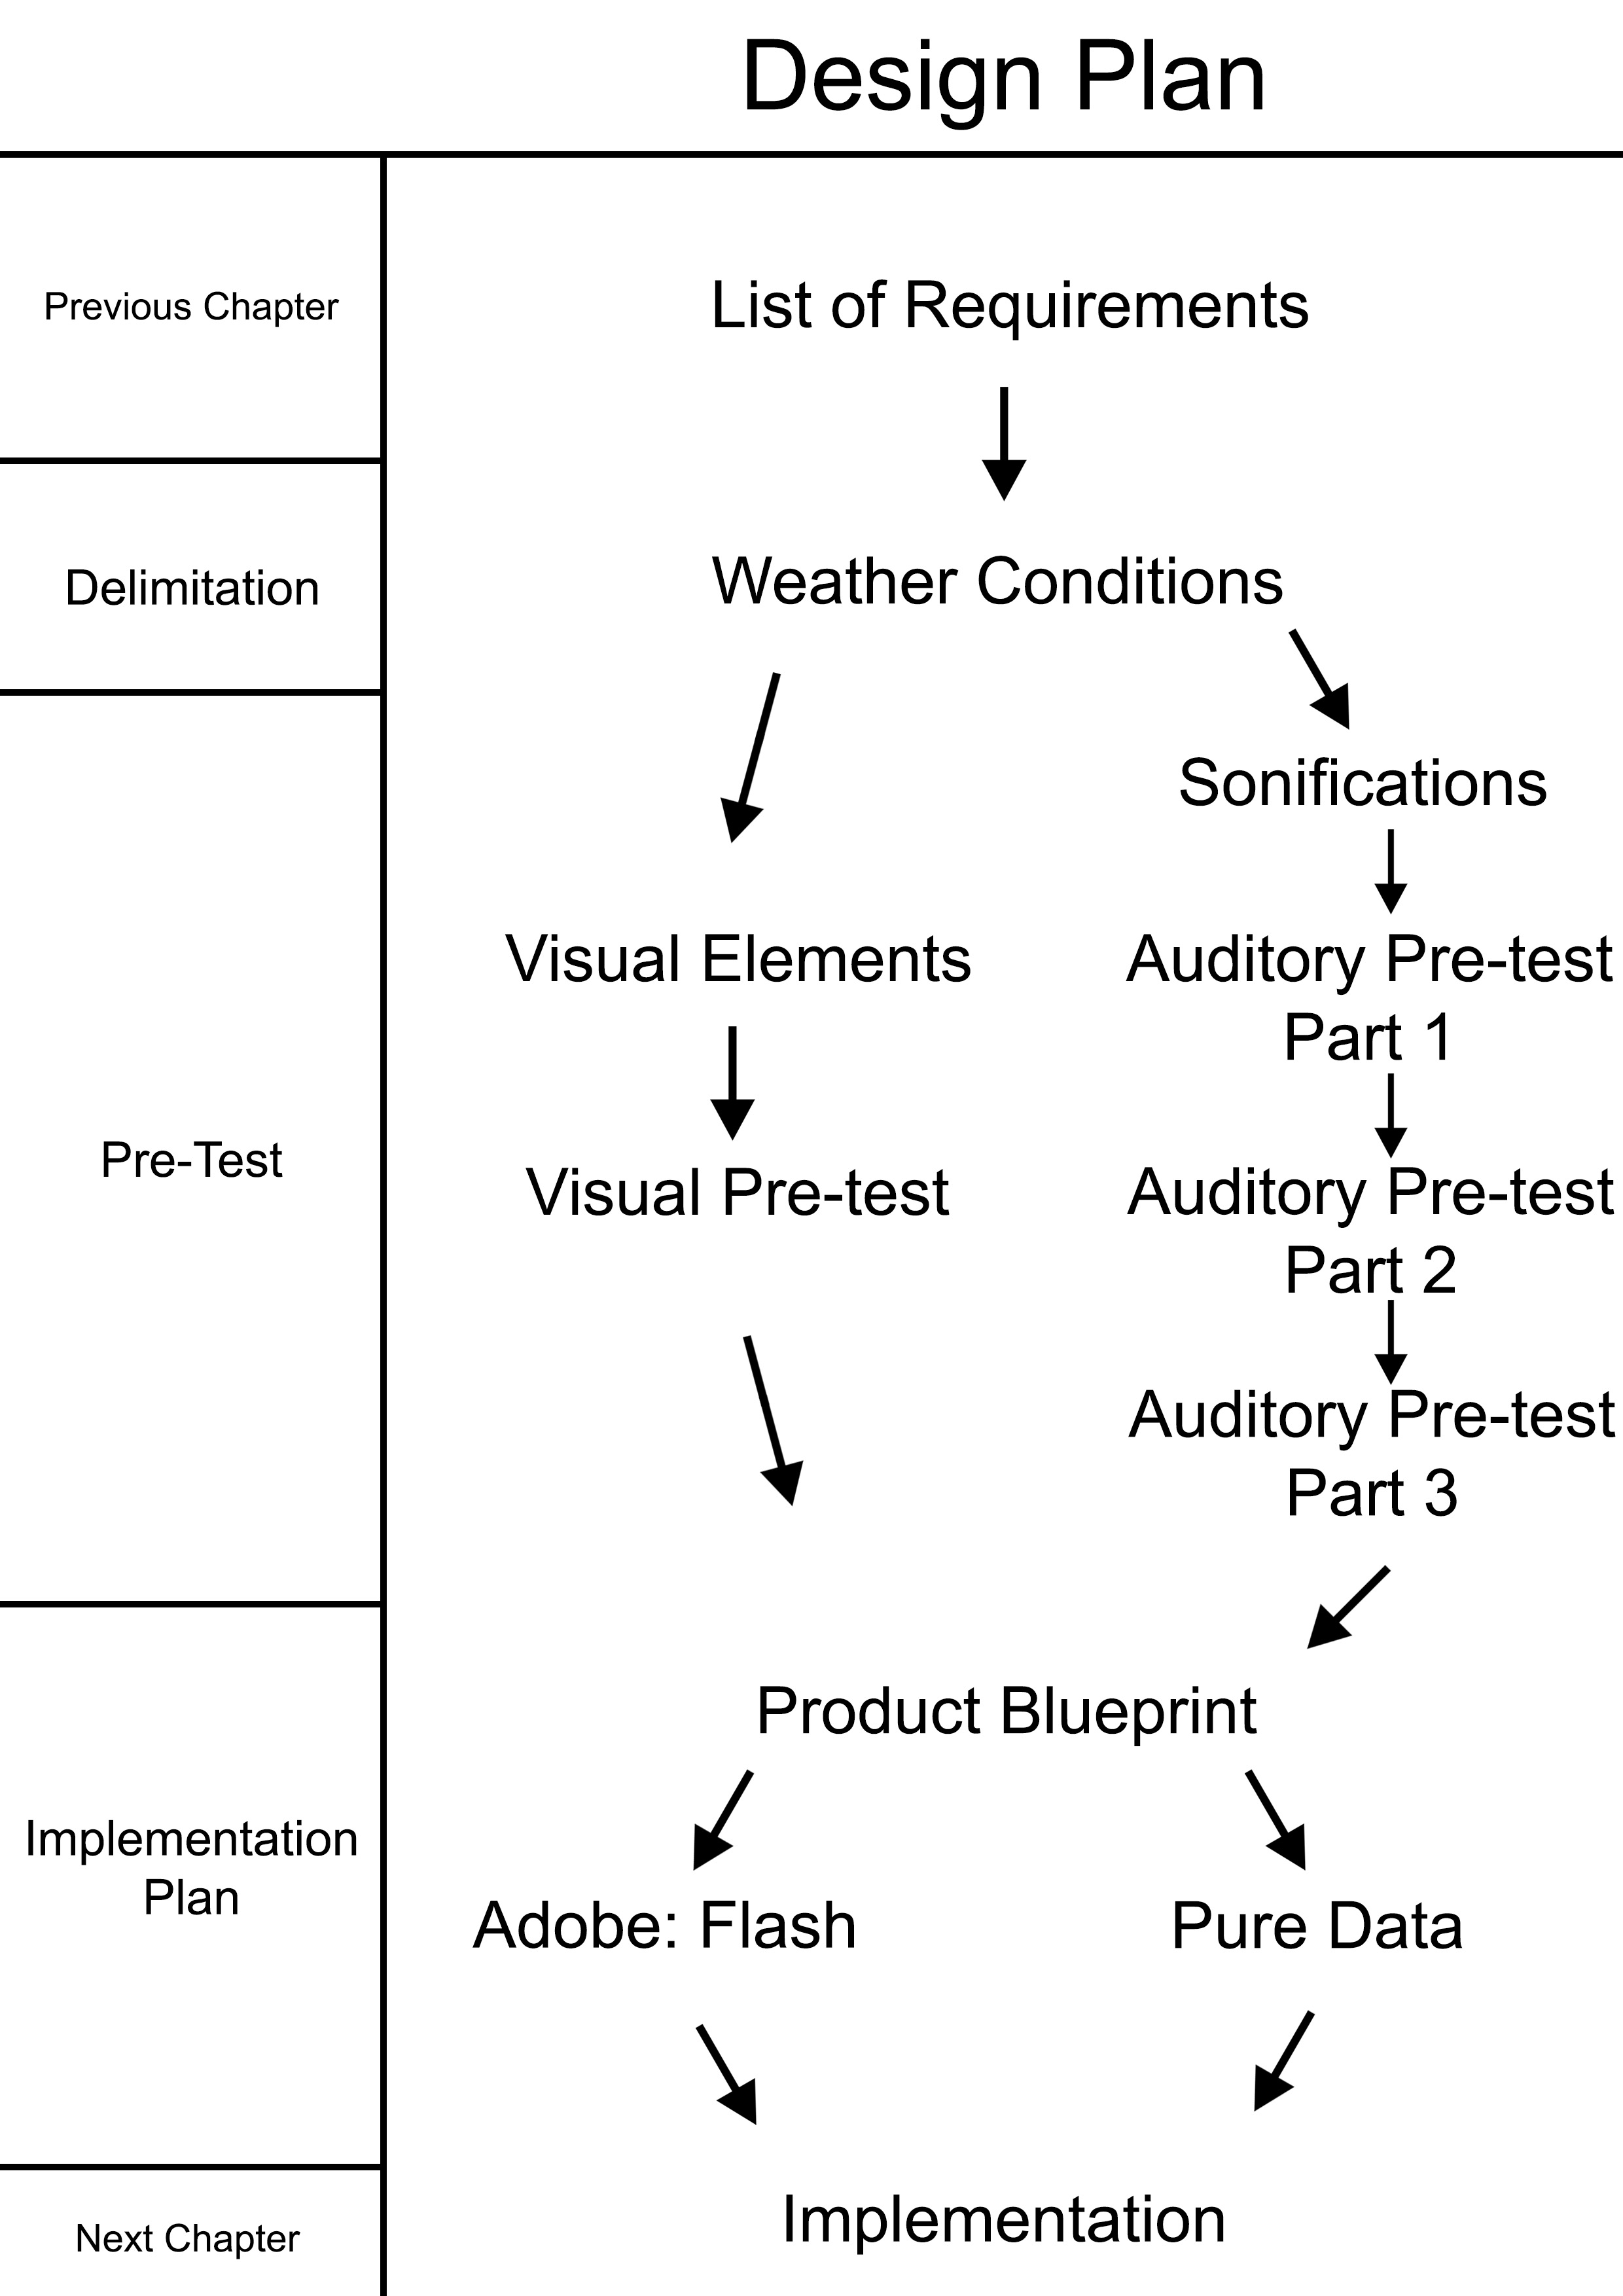
\includegraphics[width=.5\textwidth]{images/Design1.jpg}
    \caption{Plan for design process}
    \label{fig:design1}
\end{figure}


\subsection{A design to meet all the requirements} % (fold)
\label{sub:a_design_to_meet_all_the_requirements}

To get an overview of how the requirements are going to be fulfilled, the requirements have been split up into two categories. Requirements for testing and requirements for the prototype itself.

\subsubsection{Testing} % (fold)
\label{ssub:testing}

General requirements:

\begin{itemize}
    \item The prototype must contain sounds that range in different sound-parameters within the same weather category, such as varying amounts of rain.
    \item The visuals provided in testing must be based on results from either pre-testing and/or SOTA pre-analysis
    \item The sounds must have a meaning attached to them (i.e. semiosis)
    \item Symbolic representation is used to convey our message about the weather
    \item Will use the type “data exploration” of sonification to translate weather data into sound
\end{itemize}

We have decided to have a pre-test to decide on the images to be used in the prototype. 
This test involves test subjects to draw a given weather category (e.g. a drawing of certain amount of wind speed etc.). 
To determine the sounds for the prototype it was decided to make a three-step test. 

First step is to ask test participants what sounds could be used to symbolise the different weather conditions.
The second step was to make a another interview where people had to recognize the sounds that we had chosen, based upon the first pre-test. 
The last pre-test was to establish what value the test subjects associated with the specific weather conditions.

The first two pre-tests define the sounds/sonifications for the weather conditions. 
The last pre-test describes if the sonifications formulate the desired values of each weather condition.

% subsubsection testing (end)

\pagebreak
\subsubsection{Prototype} % (fold)
\label{ssub:prototype}

Program functionalities must be able to:
\begin{itemize}
    \item Import sound file
    \item Play sound file
    \item Pause sound file
    \item Change the tempo of the sound
    \item Add filters to the sounds
\end{itemize}

We have decided to use Pure data\footnote{\url{http://puredata.info/}} since we already have some knowledge in this program and know it can fulfil our requirements. 

% subsubsection prototype (end)

% subsection a_design_to_meet_all_the_requirements (end)


\subsection{Weather Conditions} % (fold)
\label{sub:weather_conditions}

There are a lot of different kinds of weather data. 
Since it is not possible to cover every single category of weather data within the projects time limit we decided to make a delimitation of the weather data to what we deemed most relevant. This decision is not based upon prior research.

Based on the research from the weather applications (See Pre-Analysis section~\ref{sub:weather_data}) the following raw weather data list was created.

\subsubsection*{Raw list of weather data} % (fold)
\label{ssub:raw_list_of_weather_data}

\begin{itemize}
     \item \textbf{Temperature/Dewpoint} - Current air temperature 2 meters above terrain.
     \begin{itemize}
         \item Day temperature
         \item Night temperature
         \item Average temperature
     \end{itemize}
     \item \textbf{Wind speed} - Average wind speed over 10 minutes, 10 meters above terrain.
     \item \textbf{Wind direction} - Average wind direction in degrees.
     \item \textbf{Air pressure} - Pressure at sea level measured i hPa (Hectopascal).
     \item \textbf{Humidity} - Current relative humidity measured 2 meters above terrain, measured in percent.
     \item \textbf{Precipitation} - Rain/sleet/snow/hail over the past ten minutes measured in mm.
     \item \textbf{Sun hours} - Hours with sun in a day.
     \item \textbf{Pollen Forecast} - The potency of the pollen. 
     \item \textbf{Sunrise / sunset} - Time of day where the sun rises and sets.
     \item \textbf{Cloud cover}
     \item \textbf{Wind chill} - The winds effect on air temperature.
     \item \textbf{Visibility} - How far can you see with clear line of sight.
     \item \textbf{UV-index} - Intensity of UV radiation.
     \item \textbf{Fronts} 
     \item \textbf{Source Regions} - Where the air is coming from.
     \item \textbf{Drought} - Risk of drought. Presented as a scale.
     \item \textbf{Downpour} - Rain in mm.
 \end{itemize}

After going through the data on the raw list we found that many of the weather categories did not fit the project. 
Therefore, we decided to only use relevant weather data that people normally would use in an everyday situation, whereof relevance is determined by us.
This delimitation is based on our research on which types of weather data there is available in the weather applications (See Pre-Analysis section~\ref{sub:weather_data}).

% subsubsection raw_list_of_weather_data (end)


\subsubsection*{List of relevant data} % (fold)
\label{ssub:list_of_relevant_data}

\begin{itemize}
     \item \textbf{Temperature/Dewpoint} - Current air temperature 2 meters above terrain.
     \begin{itemize}
         \item Day temperature
         \item Night temperature
         \item Average temperature
     \end{itemize}
     \item \textbf{Wind speed} - Average wind speed over 10 minutes, 10 meters above terrain.
     \item \textbf{Wind direction} - Average wind direction in degrees.
     \item \textbf{Humidity} - Current relative humidity measured 2 meters above terrain, measured in percent.
     \item \textbf{Precipitation} - Rain/sleet/snow/hail over the past ten minutes measured in mm.
     \item \textbf{Sun hours} - Hours with sun in a day.
     \item \textbf{Pollen Forecast} - The potency of the pollen.
     \item \textbf{Wind chill} - The winds effect on air temperature.
     \item \textbf{Visibility} - How far can you see with clear line of sight.
     \item \textbf{UV-index} - Intensity of UV radiation.
     \item \textbf{Downpour} - Rain in mm.
 \end{itemize}

Going through the weather data, we decided to make another delimitation. 
The list was further delimited based on our thoughts of what an average person would need to know in an everyday scenario, so the list of data does not necessarily represent the weather categories required to create a functional weather application with appropriate weather categories. 

% subsubsection list_of_relevant_data (end)


\subsubsection*{List of delimited weather data} % (fold)
\label{ssub:list_of_delimited_weather_data}

\begin{itemize}
     \item \textbf{Temperature/Dewpoint} - Current air temperature 2 meters above terrain.
     \begin{itemize}
         \item Day temperature
     \end{itemize}
     \item \textbf{Wind speed} - Average wind speed over 10 minutes, 10 meters above terrain.
     \item \textbf{Precipitation} - Rain/sleet/snow/hail over the past ten minutes measured in mm.
     \item \textbf{Pollen Forecast} - The potency of the pollen.
     \item \textbf{Visibility} - How far can you see with clear line of sight.
     \item \textbf{Cloud Cover.}
     \item \textbf{UV-index} - Intensity of UV radiation.
     \item \textbf{Downpour} - Rain in mm.
 \end{itemize}

% subsubsection list_of_delimited_weather_data (end)


\subsubsection{Categories} % (fold)
\label{ssub:categories}


We did not use Continuous Sonification as specified in the analysis. (See analysis section~\ref{ssub:sonification_techniques}), because it is hard for people to interpret numbers, for example: \enquote{Could you make a sound based on a temperature of 12 degrees?}. 
Since it is not possible for us to go through every degree of e.g. temperature, the numbers were converted into three categories: Low, Medium and High. 
We also decided that the weather data "Pollen" and "Visibility", should act like a warning indicator. 
This means that the sound should only be played above or below a specific value.
This decision was made since there is no reason to warn users about weather conditions that might affect the user when there is none. 
In this case "Pollen" will be played when there is a high amount of pollen, and "Visibility" will be played when there is low visibility.

When the values had been decided , the values had to be assigned. We are getting our Low, Mid and High value from DMI\footnote{\url{http://www.dmi.dk/vejr/til-lands/byvejr/by/vis/DK/1000/K\%C3\%B8benhavn,\%20Danmark}}. The values are estimates of low, medium and high based on the data from DMI.

\begin{table}[!h]
\centering
\begin{tabular}{l | l | l | l}
Category & Low & Medium & High \\
\hline \hline
Temperature & 0'C & 15'C & 30'C \\
Wind Speed & 5 m/s & 17 m/s & 32 m/s \\
Pollen Forecast & 0 - 30 & & 30 - 100 \\
Visibility & 10 m & & 10 km \\
Downpour & 0 mm & 3 mm & 10 km \\
UV-index & 3 & 3 - 6 & 7 - 8 
\end{tabular}
\caption{Category values}
\label{tab:category_values}
\end{table}
% subsubsection categories (end)

% subsection weather_conditions (end)

\subsection{Visual pre-test} % (fold)
\label{sub:visual_pre_test}

A pre-test was done to identify the common visual associations often used with the weather forecasts, these associations will form a basis for the visual implementations. 
The visual implementation will contain images of certain weather conditions that people should find intuitive.

The test took the form of a simple interview where the subject was asked to draw certain weather conditions.

Because the test has no target group other than people who have at some point checked a weather forecast, the test will be conducted using accidental sampling.
accidental sampling selects every subject in the test from a greater group of subjects (the target group) completely at random. 
Every subject has an equal chance to get picked to do the survey.

The selected subjects would be given a piece of paper with three empty frames. 
The subject was then asked to draw the first thing that came to mind when told about a weather condition. 
A sample question could be: \enquote{draw the first thing that comes to mind when i tell you that it is 30*C outside}. 
The subject would then draw their association. 
The subject would then be asked to make another drawing of the same weather condition but with a different value. 
i.e. if the subject had first been asked to draw a hot day, they would then be asked to draw a cold day and then an average day.

5 people for each weather condition was asked to participate, 35 in total. 
The complete drawing sheet and answers to the survey can be found in appendix~\ref{sec:visual_pre_test_raw_results}.

\begin{table}[!htbp]
    \centering
    \begin{tabular}{l | l | l | l}
    Condition & Value & Possible solution & Alternate solution \\
    \hline \hline
    Temperature & Low & Snowflake, snow &  \\
    & Medium & Average clothing \\
    & High & Sun and beach & Thermometer \\
    \hline
    Downpour & Low & Sunny & Clouds, no rain \\
    & Medium & Clouds with rain & \\
    & high & Clouds with much rain & \\
    \hline
    Wind speed & Low & Tree/Flag, no movement & \\
    & Medium & Tree/flag, some movement & \\
    & High & Tree/man, much movement & \\
    \hline
    Pollen & Low & Man, happy/smiling & \\
    & Medium & Man, Sneezing & \\
    & High & Man w. runny nose, red eyes, itching & \\
    \hline
    Visibility & Low & Window, gray outside & \\
    & Medium & Gray colors & cloudy \\
    & High & Clear day, sun & \\
    \hline
    Cloud cover & Low & Clear day, sun & \\
    & Medium & Few Clouds & \\
    & High & Overcast & \\
    \hline
    UV-index & Low & Cloudy day & \\
    & Medium & Clouds, sun & \\
    & High & Sun, no clouds & \\
    \end{tabular}
    \caption{Possible visual implementations}
    \label{tab:visual_pre_test}
\end{table}

Table~\ref{tab:visual_pre_test} shows the possible solutions for the visual implementation based on the acquired results.
The drawings were analyzed for common traits within the same condition and value, i.e. if two or more drawings of the same condition and value would contain a person, this would be interpreted as a possible common association and be included as possible solution.

% subsection visual_pre_test (end)

\FloatBarrier
\subsection{Sound pre-test} % (fold)
\label{sub:sound_pre_test}
The idea of the pre-test is to determine what sounds to choose when looking for the optimal choice of sounds to use the designated sonifications of each weather condition. 
We will go through a three step audio pre-test that will provide us with the information we need. 
The first step is meant to give us insight about what sound to use. 
The second step is to test these previously mentioned sounds to see if people recognize what it is meant to represent. 
The third step is to play the sounds to the test subjects and then ask what weather data these sounds represent, in a setting where we have already specified the weather category, to figure out if the specified sound also formulates the designated value of the weather condition.

\subsubsection{Audio Pre-Test - Part One} % (fold)
\label{ssub:audio_pre_test_part_one}
This first part of the pre-test was meant to give an idea of what sounds to use according to the feedback given from interviews. 
We then provide our own thoughts in addition to determine what the sounds should be.

\paragraph{Purpose} % (fold)
\label{par:purpose} 
\hspace{0pt} \\
Determine what sounds to use in each of the weather condition categories as specified in the list of delimited weather data. See \ref{ssub:list_of_delimited_weather_data}

% paragraph purpose (end)

\paragraph{Description} % (fold)
\label{par:description}
\hspace{0pt} \\
Part one was performed by interviewing people randomly selected around the AAU campus. 
This part of the pre-test contains questions about how the testers would describe the different weather categories with a sound or a scenario, both for high and low values of the specific weather conditions. 
This information is then used to acquire/develop the sounds for the pre test, where the actual sounds will be tested to see if they represent the answers acquired from this test.

\begin{tabular}{l l}
Amount of participants: & 12 test participants \\
Test subject sampling: & Convenience sampling: Aalborg University students. \\
Estimated length of test: & Around 10 min per test subject. \\
Test location: & Area on and around Aalborg university. \\
Date and time: & When appropriate.
\end{tabular}

% paragraph description (end)

\paragraph{Results} % (fold)
\label{par:results}
\hspace{0pt} \\
See appendix~\ref{sub:pre_test_1_results} for results.

These results have been placed together for each category, where you can see answers for both high and low values. 

% paragraph results (end)

\paragraph{Evaluation} % (fold)
\label{par:evaluation}
\hspace{0pt} \\
When analyzing the data that has been gathered, it was seen that most of the categories have the same answers. 
Our sounds were based on a mix of how the majority wanted the sounds to be like and what we believed could be a recognizable sound. 
The following is an overview of our thought process. 

\subparagraph{Temperature} % (fold)
\label{subp:temperature}
\emph{High:} We noticed that a high pitched sound was a frequent answer among the participants. We went with this in mind when choosing the soun. 
The sound that we ended up choosing, was inspired by one of the participants that answered \enquote{a boiling kettle}. \newline
\emph{Low:} The majority answered \enquote{breaking ice} and \enquote{snow}, but since we are using that for Precipitation - Snow it is not an option. 
We instead went with the \enquote{teeth grinding} sound.
% subparagraph temperature (end)

\subparagraph{Wind Speed} % (fold)
\label{subp:wind_speed}
\emph{High:} A \enquote{high wind gust} seemed to be the most common answer, so that is what we went with.
\emph{Low:} A \enquote{low wind gust} seemed to be the most common answer, so that is what we went with.
% subparagraph wind_speed (end)

\subparagraph{Precipitation} % (fold)
\label{subp:precipitation}
\emph{Rain:} All the answers to this were \enquote{rain}, so we went with rain as our sound.
\emph{Snow:} Most of the answers to this were \enquote{snow}, but since snow does not have a sound then we went with footsteps in the snow.
\emph{Hail:} All the answers to this were \enquote{hail}, so we went with hail as our sound.
% subparagraph precipitation (end)

\subparagraph{Pollen Forecast} % (fold)
\label{subp:pollen_forecast}
\emph{High:} \enquote{A sneeze} was the most common answer, so that is what we chose as our sound.
\emph{Low:} Because we are going with pollen as a warning indicator this question was only stated to satisfy our curiosity. 
The test participants did not give any real responses to this question. 
% subparagraph pollen_forecast (end)

\subparagraph{Visibility} % (fold)
\label{subp:visibility}
\emph{Low:} Most of the people we asked described a foggy scenario as seen in movies. 
Since this is the scenario most people think of, we chose a \enquote{fog horn} sound to remind them of this scenario in the hopes that they would associate it with a foggy day.
% subparagraph visibility (end)

% paragraph evaluation (end)

% subsubsection audio_pre_test_part_one (end)


\subsubsection{Audio Pre-Test - Part Two} % (fold)
\label{ssub:audio_pre_test_part_two}

\paragraph{Purpose} % (fold)
\label{par:pre_test_2_purpose}
\hspace{0pt} \\
The second part of the pre-test is based upon the results given from pre test 1 (See section~\ref{ssub:audio_pre_test_part_one}). 
The results has been evaluated, and sounds that could be used as a sonification of the specific weather conditions has been found/developed. 
The following test is conducted as we want to ensure that the chosen sounds actually represent the results from the previous test and can be used in the designated prototype. 
The test will elaborate upon the sounds and will make it possible to evaluate whether the sounds are understood or not, and what the test subjects think that the sounds intuitively implies.
% paragraph purpose (end)

\paragraph{Description} % (fold)
\label{par:pre_test_2_description}
\hspace{0pt} \\
The procedure of the test was conducted in the following manner. 
A single test subject was asked to listen to the acquired/constructed sounds, and was then asked to write down what he/she relates to the sound e.g. what the subject thought of the sound actually implies. 
The test subject was given no prior information to the test, and was unaware of everything but the test procedure.
This ensured that the test subject was given no information that could be used to assume anything based upon the sounds and somewhat bias the results, as we were looking for the intuitive understanding of the presented sounds.

\begin{tabular}{l l}
Amount of participants: & 10 test participants \\
Test subject sampling: & Convenience sampling \\
Estimated length of test: & 10 min per test subject. \\
Test location: & Area on and around Aalborg university. \\
Date and time: & When appropriate.
\end{tabular}

% paragraph description (end)

\paragraph{Results} % (fold)
\label{par:pre_test_2_results}
\hspace{0pt} \\
See appendix~\ref{sub:pre_test_2_results} for the acquired test results.

\enquote{List of sounds} represents the sounds that were played to each individual test subject in that specific order.
\enquote{Test x} represents answers written down from each test participant in each column, where the data represents the denoted answer from the test participant.
The right sided column to each test section represents the interpretation of results.

The result interpretations are divided into three categories: \newline
\textbf{Correct} - Represents a correct answer. \newline
\textbf{Correct()} - Represents an answer that is associated with the correct answer, as decided by us, and is therefore marked as correct. 
The associations are deemed correct by us and does not represent a scientific decision. \newline
\textbf{Incorrect} - Represents an incorrect answer. 
Either the sound was not guessed, indicated by \enquote{-}, in the test results, or the responses was not in any way associated with the sound, as deemed by us.

% paragraph results (end)
\pagebreak[3]
\paragraph{Evaluation} % (fold)
\label{par:pre_test_2_evaluation}
\hspace{0pt} \\
Table \ref{tab:pre_test_2_evaluation} illustrates the amount of correct answers in percentages.

\begin{table}[!hb]
\centering
\begin{tabular}{l l r c}
   & Sound &  Answered correctly & \\
\hline
1. & Hail - Downfall hail & 70\% & 7/10 \\
2. & Rain - Downfall rain & 100\% & 10/10 \\
3. & Snow - Downfall snow & 10\% & 1/10 \\
4. & Birds - Downfall nothing & 60\% & 6/10 \\
5. & Horn - Fog & 90\% & 9/10 \\
6. & Sneeze - Pollen & 90\% & 9/10 \\
7. & Kettle - High temperature & 90\% & 9/10 \\
8. & Clattering Teeth - Low temperature & 0\% & 0/10 \\
9. & Small breeze - Medium temperature & 70\% & 7/10 \\
10. & Wind - Wind speed & 100\% & 10/10
\end{tabular}
\caption{Pre-test 2 evaluation}
\label{tab:pre_test_2_evaluation}
\end{table}

\begin{enumerate}
    \item \textbf{Hail} - The majority of test subjects answered \enquote{hail}, which was the desired implication of the sound. 
    We suspect that when the test subjects are aware of the subject, being weather - and thereafter will have to guess what the sound implies - the sound will suffice.
    \item \textbf{Rain} - All test subjects answered correctly, therefore the sound is deemed to require no alterations or changes.
    \item \textbf{Snow} - A low amount of test participants, around 10\%, was able to associate the sound with snow as intended. We therefore chose to replace the sound.
    \item \textbf{Birds} - A majority of 60\% answered correctly. This indicates that while most answers correct, adjustments might ensure that a larger percentage of test subjects will answer correct. Plausible alterations will be decided by us.
    \item \textbf{Horn} - A Majority of 90\% answered correctly. Therefore no alterations will be made.
    \item \textbf{Sneeze} - A Majority of 90\% answered correctly. Therefore no alterations will be made.
    \item \textbf{Kettle} - A Majority of 90\% answered correctly. Therefore no alterations will be made.
    \item \textbf{Teeth} - No test participants were able to answer correctly. Therefore we will replace the sound.
    \item \textbf{Small breeze} - The majority of 70\% was able to answer correctly. Adjustments will be made, and might ensure that a larger percentage of the subjects will be able to answer correct. Plausible alterations will be decided by us.
    \item \textbf{Wind} - All test subjects answered correctly, therefore the sound is deemed to require no alterations or changes.
\end{enumerate}

% paragraph evaluation (end)

% subsubsection audio_pre_test_part_two (end)

\subsubsection{Audio Pre-Test - Part Three} % (fold)
\label{ssub:audio_pre_test_part_three}
Since the previous part of the pre-test we replaced the LowTemp sound (Teeth) with a new sound that has been tested around the campus and is being deemed ready for use. 
A small delimitation has also been made to downpour. 
It now only covers rain since we encountered a problem that we didn’t think about at the early stages. 
The problem was that we designed downpour to be changed by play speed of the sound, and the only sound capable of being modified in this manner is rain.

Now that every sound has been deemed ready for use, we are able to proceed into the third step of the pre-test. 
In this step we are going to play the sound and give information about what weather category it is. 
We then want our testers to answer what weather data type they believe the sound represents.  

\paragraph{Purpose} % (fold)
\label{par:pre_test_3_purpose}
\hspace{0pt} \\
The purpose of this part of the pre-test is to make sure that our sounds are recognisable with a weather data type when combined with a weather category.
% paragraph purpose (end)

\paragraph{Description} % (fold)
\label{par:pre_test_3_description}
\hspace{0pt} \\
\begin{tabular}{l l}
Amount of participants: & 10 test participants \\
Test subject sampling: & Convenience sampling \\
Estimated length of test: & 15 min per test subject. \\
Test location: & Ballerup, Albertslund, and Aalborg university. \\
Date and time: & When appropriate.
\end{tabular}
% paragraph description (end)

\paragraph{Results} % (fold)
\label{par:pre_test_3_results}
\hspace{0pt} \\
See appendix \ref{sub:pre_test_3_results} for results.

On this list it can be seen what each test person answered to the sounds.
% paragraph results (end)

\paragraph{Evaluation} % (fold)
\label{par:pre_test_3_evaluation}
\hspace{0pt} \\
Most of our sounds were recognisable and provided the people testing with the intended information. \newline
There were a few sounds (listed below) that gave us some negative data.

\subparagraph{TempMed:} % (fold)
\label{subp:tempmed_}
People gave many different answers for this sound. 
This is a problem and this sound has to be replaced and tested once more.
% subparagraph tempmed_ (end)

\subparagraph{Pollen:} % (fold)
\label{subp:pollen_}
Most of the people got the correct weather category but some also answered \enquote{cold}. 
Since it is a sneeze this is something that we should have expected. 
We will try to modify the to make sure that test participants make a clearer association to pollen. 
% subparagraph pollen_ (end)

\subparagraph{Fog:} % (fold)
\label{subp:fog_}
All the people that answered the question got the answer correct. 
However, we also had some people who were unable to answer the question. 
We conclude that they might know what the sound is, but they do not manage to connect it into that foggy scenario that we imagined people would in the first part of the pre-test.
% subparagraph fog_ (end)

% paragraph evaluation (end)

After making the proper adjustments to the sounds, we feel that we are at this point ready to implement them, and use them for further testing.

% subsubsection audio_pre_test_part_three (end)

% subsection sound_pre_test (end)

\FloatBarrier
\subsection{Product Blueprint} % (fold)
\label{sub:product_blueprint}

Now that the visual and auditory elements have been determined, it is time for us to plan how to make use of the acquired data.

\subsubsection{Visual Elements} % (fold)
\label{ssub:visual_elements}

The visual design is based on the table from the visual pre-test (Table~\ref{tab:visual_pre_test}). We use the information from our user pre-test, where to test subjects had to draw how they imagined a certain weather condition to be illustrated, to come up with similar illustrations for weather conditions in the prototype.

% subsubsection visual_elements (end)


\subsubsection{Audio elements} % (fold)
\label{ssub:audio_elements}

When the different sounds for weather categories were in place, the next step was to figure out how to make these sounds fit into our value categories. 
Most of the sounds can be placed and played under the fitting values, but rain (Downpour) and wind speed had to be changed in order to let people know if it had a low, medium or high value.
In order to change these sounds we decided to use Pure Data.
With Pure Data it was possible to change the speed of the sound and add filters so the sounds that were able to fit into our value categories.

Here are the Pure Data objects we will use for the implementation:

\paragraph{Band Pass Filter} % (fold)
\label{par:band_pass_filter}

Band Pass Filter also called [bp~] in Pure Data, is a filter that only allows some range of frequencies between the highest and lowest. 
It has three inputs. 
The first one is the input from the audio. 
The second input is for the center frequency that will be allowed to pass. 
The third input is the resonance, which determines how wide the ranges of frequencies that are allowed to pass through the filter are. 
The function is that the center frequency will be unchanged, but the frequencies, higher or lower, will be reduced or removed from the sound.

% paragraph band_pass_filter (end)


\paragraph{Sample} % (fold)
\label{par:sample}

A sample refers to a value or multiple values that is set to a point in time.

% paragraph sample (end)


\paragraph{Metro} % (fold)
\label{par:metro}

An object that keeps calling after a specific amount of time (in milliseconds).

% paragraph metro (end)
    

\paragraph{Phasor} % (fold)
\label{par:phasor}

A phasor is a representation of a sinusoidal function. 
This function is based on three factors, A is the functions amplitude, $\omega$ is the frequency and $\theta$ is the phase.  

\begin{equation}
    A * \cos(\omega t + \theta)
\end{equation}

We use the phasor by sending in our normal frequency. This will change the sinusoidal wave and by that change the play speed of samples.

% paragraph phasor (end)

\paragraph{Soundfiler} % (fold)
\label{par:Soundfiler}

A soundfiler is an object that reads and writes floating point arrays to binary soundfiles. This is something we might have a use for when we import the sounds into Pure Data.

% paragraph phasor (end)

\subsubsection{How the sound will be implemented in Pure Data} % (fold)
\label{ssub:how_the_sound_will_be_implemented_in_pure_data}

The way the sound will be implemented in pure data:

\begin{enumerate}
    \item Input Sound
    \item Array / Sample
    \item Determine Sample Speed
    \item Phasor
    \item Merge Array and Sample Speed
    \item Fliter (if required)
    \item Output Sound
\end{enumerate}

First step is to make sure that the sound will be imported into the program. 
Second step is to send the sound into an array that will split the sound into samples. 
The third step is to detect how fast the samples normally are going to be played in order to create the same sound. 
The fourth step is sending the normal frequency into a Phasor. 
The fifth step is to merge the play speed from the phasor with the array with the samples. 
This will create the sound based on the play speed that has been changed. 
The sixth step is only to be implemented if a filter is required for the sound. 
The seventh and last step is the output sound that have been going through all the new changes and will now sound differently.

Now that all of sounds have been decided and the design of our product complete, we can now enter the implementation stage. 

% subsubsection how_the_sound_will_be_implemented_in_pure_data (end)

% subsubsection audio_elements (end)

% subsection product_blueprint (end)

% section design (end)